%"###############################################
%
% Classification supervisée
%
%###############################################

% VPPBS: variables post-op à 12 mois
%
%###############################################

\subsubsection{VPPBS: IPSS à 12 mois}
\begin{figure}[H]
\centering
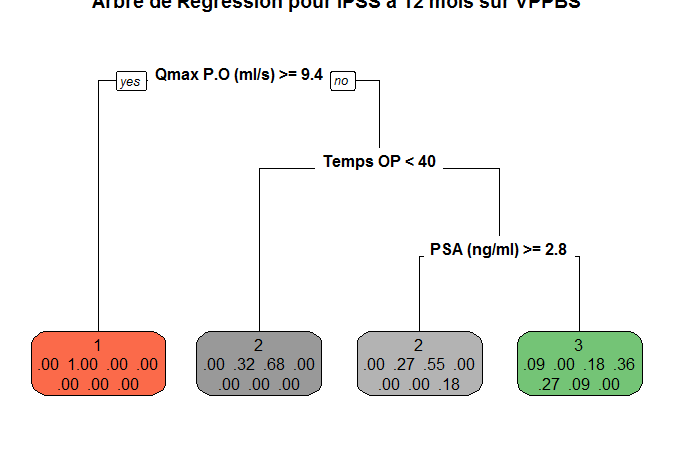
\includegraphics[width=0.75\textwidth]{../Fig/VPPBS/vppbs-regtree-ipss12.png}
\caption{VPPBS: Arbre de régression pour IPSS à 12 mois}
\label{fig-vppbs-regtree-ipss12}
\end{figure}

\begin{figure}[H]
\centering
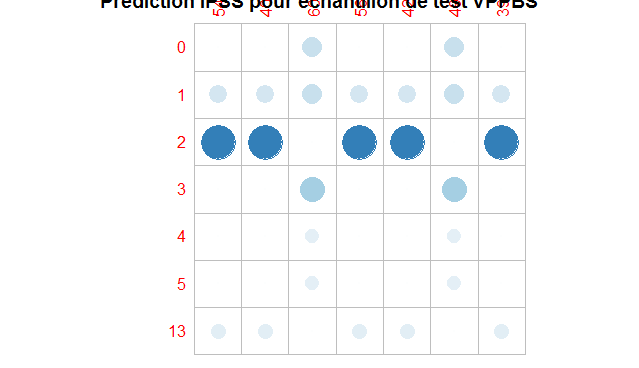
\includegraphics[width=0.75\textwidth]{../Fig/VPPBS/vppbs-regtree-predict-ipss12.png}
\caption{VPPBS: Prévision pour IPSS à 12 mois}
\label{fig-vppbs-regtree-predict-ipss12}
\end{figure}

\subsubsection{VPPBS: QoL à 12 mois}

\begin{figure}[H]
\centering
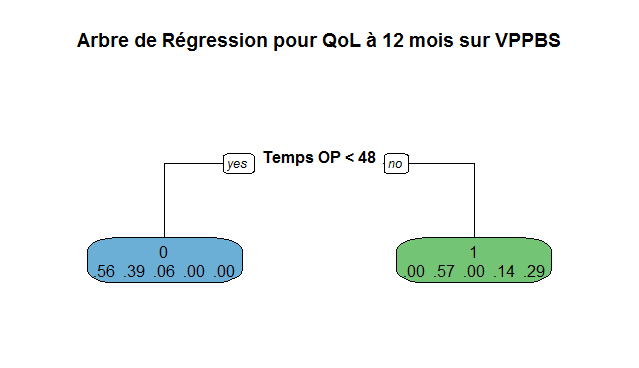
\includegraphics[width=0.75\textwidth]{../Fig/VPPBS/vppbs-regtree-qol12.png}
\caption{VPPBS: Arbre de régression pour QoL à 12 mois}
\label{fig-vppbs-regtree-qol12}
\end{figure}

\begin{figure}[H]
\centering
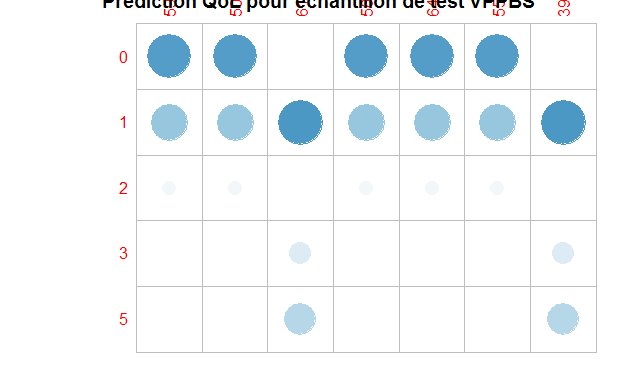
\includegraphics[width=0.75\textwidth]{../Fig/VPPBS/vppbs-regtree-predict-qol12.png}
\caption{VPPBS: Prévision pour QoL à 12 mois}
\label{fig-vppbs-regtree-predict-qol12}
\end{figure}


\subsubsection{VPPBS: Qmax à 12 mois}

\begin{figure}[H]
\centering
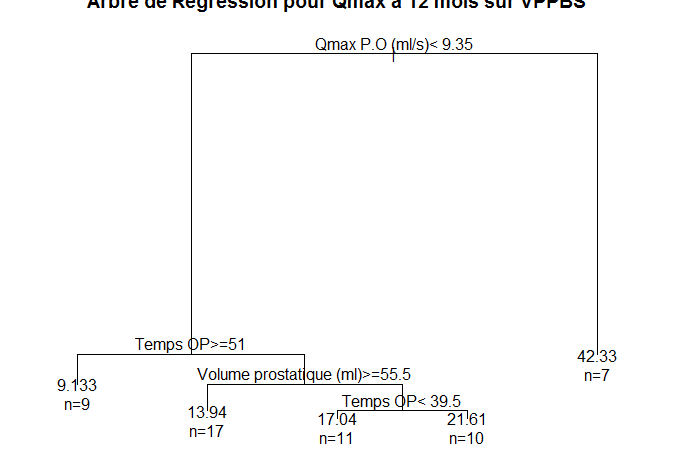
\includegraphics[width=0.75\textwidth]{../Fig/VPPBS/vppbs-regtree-qmax12.png}
\caption{VPPBS: Arbre de régression pour Qmax à 12 mois}
\label{fig-vppbs-regtree-qmax12}
\end{figure}

\begin{figure}[H]
\centering
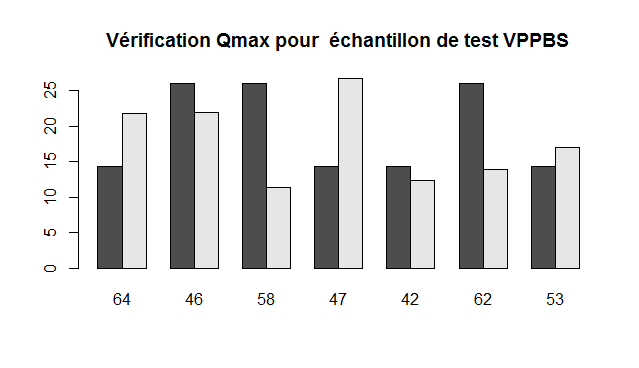
\includegraphics[width=0.75\textwidth]{../Fig/VPPBS/vppbs-regtree-test-qmax12.png}
\caption{VPPBS: Evaluation des prévisions pour Qmax à 12 mois}
\label{fig-vppbs-regtree-test-qmax12}
\end{figure}

